% Welcome! This is the unofficial University of Udine beamer template.

% See README.md for more informations about this template.

% This style has been developed following the "Manuale di Stile"
% (Style Manual) of the University of Udine. You can find the
% manual here: https://www.uniud.it/it/ateneo-uniud/ateneo-uniud/identita-visiva/manuali-immagine-stile/manuale-stile

% Note: for some reason, the RGB values specified in the manual
% do NOT render correctly in Beamer, so they have been redefined
% for this document using the high level chromo-optic deep neural 
% quantistic technology offered by Microsoft Paint's color picker.

% We defined four theme colors: UniBrown, UniBlue, UniGold
% and UniOrange. For example, to write some uniud-brownish
% text, just use: \textcolor{UniBrown}{Hello!}

% Note that [usenames,dvipsnames] is MANDATORY due to compatibility
% issues between tikz and xcolor packages.

\documentclass[usenames,dvipsnames]{beamer}
\usepackage[utf8]{inputenc}
\usepackage{verbatim}
\usepackage{multicol}
\usepackage{cases}
\usepackage{cancel}
\usetheme{uniud}
%set depth of Outline
\setcounter{tocdepth}{2}
%%% Bibliography
\usepackage[style=authoryear,backend=biber]{biblatex}
\addbibresource{bibliography.bib}

% Author names in publication list are consistent 
% i.e. name1 surname1, name2 surname2
% See https://tex.stackexchange.com/questions/106914/biblatex-does-not-reverse-the-first-and-last-names-of-the-second-author
\DeclareNameAlias{author}{first-last}

%%% Suppress biblatex annoying warning
\usepackage{silence}
\WarningFilter{biblatex}{Patching footnotes failed}

%%% Some useful commands
% pdf-friendly newline in links
\newcommand{\pdfnewline}{\texorpdfstring{\newline}{ }} 
% Fill the vertical space in a slide (to put text at the bottom)
\newcommand{\framefill}{\vskip0pt plus 1filll}


\title[Weekly meeting]{Weekly meeting}
\date[Nov 13, 2024]{Nov 11, 2024}
\author[Chengxin Liao]{
  Chengxin Liao
  \pdfnewline
  \texttt{liaocx@ihep.ac.cn}
}
\institute{Department of Physics, Shandong University}

\begin{document}

\begin{frame}
\titlepage
\end{frame}

\begin{frame}{Outline}
\tableofcontents
\end{frame}

\section{Introduction}
\subsection{event selection}
\begin{frame}
\frametitle{Introduction}
\framesubtitle{event selection}
\begin{columns}
    \column{0.6\textwidth}
    \raggedright
    Selection
	\begin{enumerate}[\textbullet]
    \item lep-had channel:nTaus$\geq$1;nLeps$\geq$1
    
    \item had-had channel:nTaus$\geq$2;nLeps=0
    
    \item MET$\geq$ 200; pass MET trigger
    
    \item $1\leq nBaseJet\leq 8$
     
    \item b-veto
    
    \item OS
    \end{enumerate}
    \vskip 0.2cm
    
%    For sig/bkg plot, both bkg and signal distribution are normalized to 1.
%    
    Both data and bkg are sourced from run2(1516, 17, 18).
%    
%    Kinematic variables with better separation power are marked with black box.
    \column{0.5\textwidth}
    
    \raggedleft
    \begin{figure}
    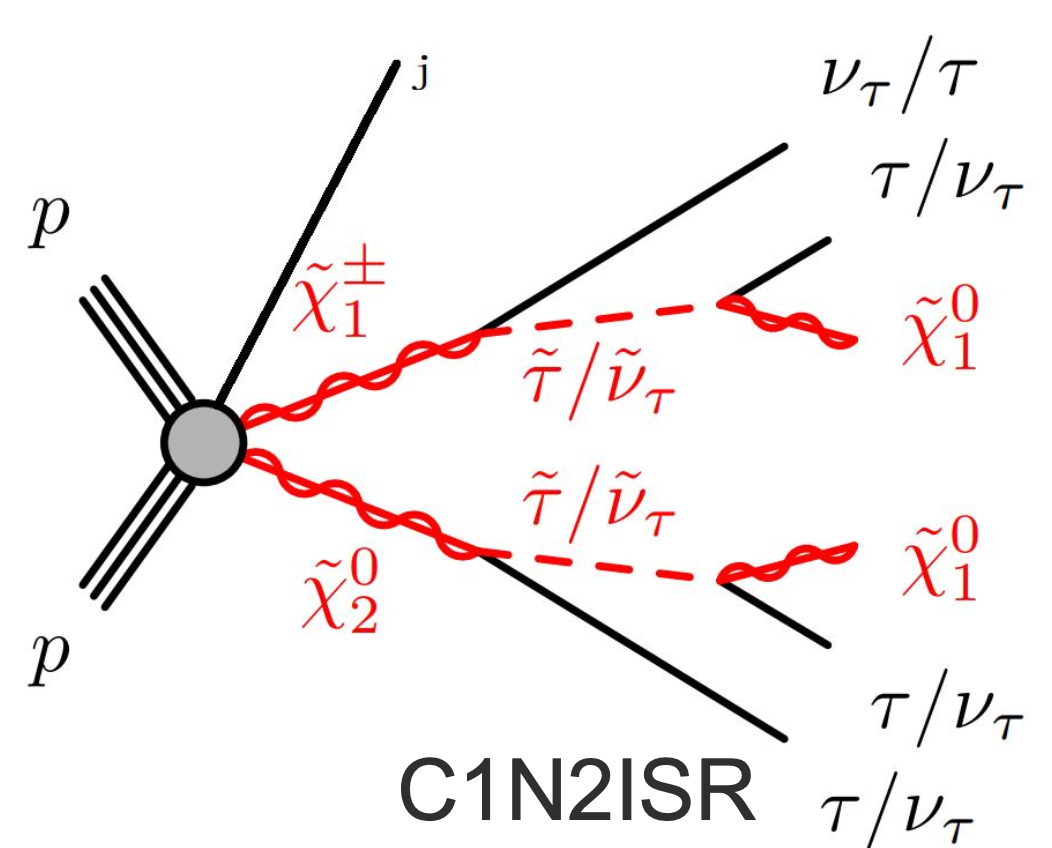
\includegraphics[width = 0.5\textwidth]{graphics/Feynman diagram.png}
    \end{figure}
 \end{columns}

\end{frame}

\subsection{LH kinematic distribution}
\begin{frame}
	\frametitle{kinematic distribution}
	\framesubtitle{LH:$p_T$}
For sig/bkg, both bkg and signal distribution are normalized to 1. Kinematic variables with better separation power are marked with black box.

% 第一行
    \begin{minipage}{0.32\textwidth}
        \centering
        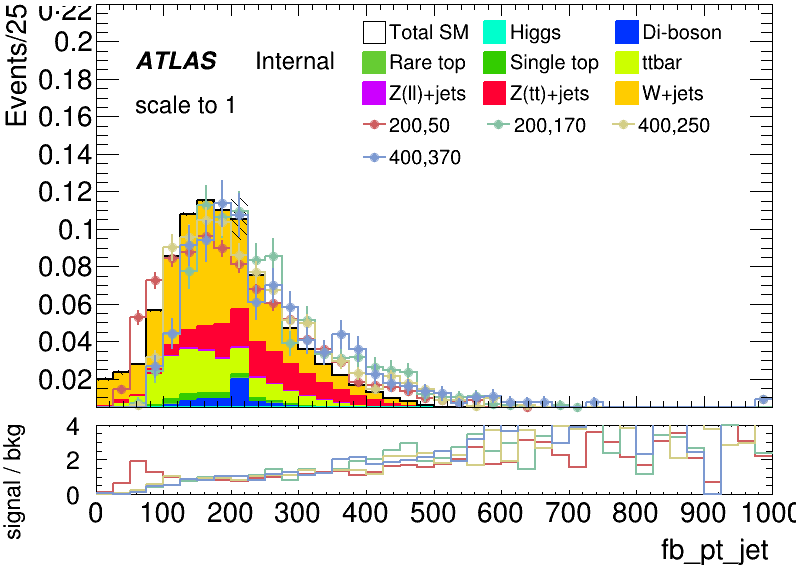
\includegraphics[width=\textwidth]{graphics/LH_met_sig/LH_fb_pt_jet_norm.png}
    \end{minipage}
    \hfill
    \begin{minipage}{0.32\textwidth}
        \centering
        \setlength{\fboxsep}{0pt} % 边框与图片的距离
        \setlength{\fboxrule}{1pt} % 边框的粗细
        \fbox{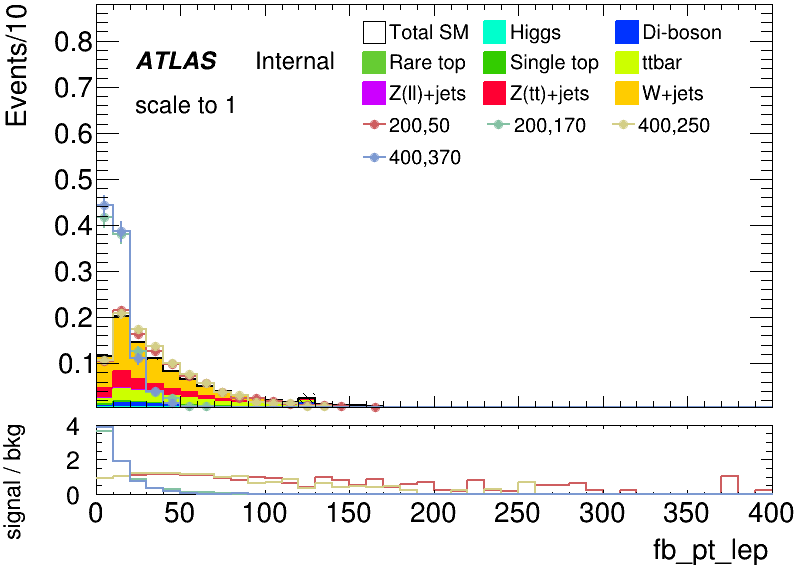
\includegraphics[width=\textwidth]{graphics/LH_met_sig/LH_fb_pt_lep_norm.png}}
    \end{minipage}
    \hfill
    \begin{minipage}{0.32\textwidth}
        \centering
        \setlength{\fboxsep}{0pt} % 边框与图片的距离
        \setlength{\fboxrule}{1pt} % 边框的粗细
        \fbox{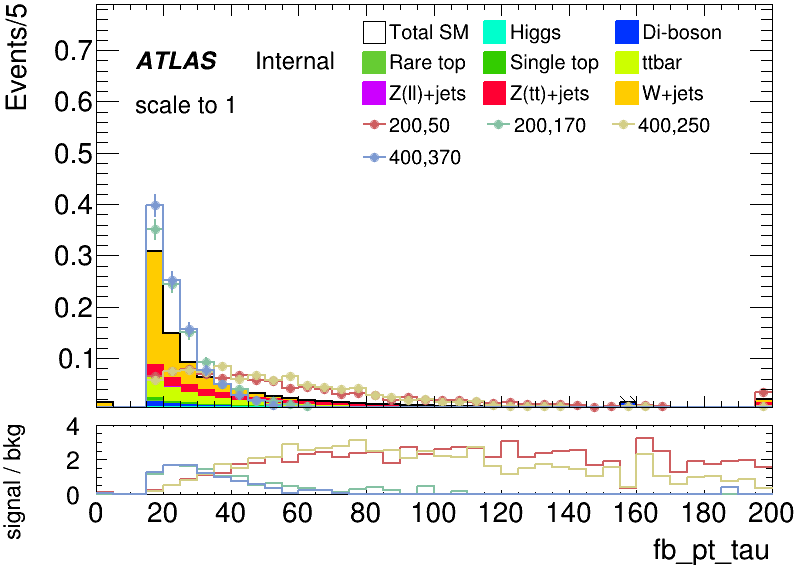
\includegraphics[width=\textwidth]{graphics/LH_met_sig/LH_fb_pt_tau_norm.png}}
    \end{minipage}
    
    \vspace{0.5cm} % 图片之间的竖直间距
    
    notice: t1 is leading tau, t2 is leading lep, j is leading jet, x is MET.
\end{frame}

\begin{frame}
  \frametitle{kinematic distribution}
  \framesubtitle{LH:MET}
    \begin{minipage}{0.5\textwidth}
        \centering
        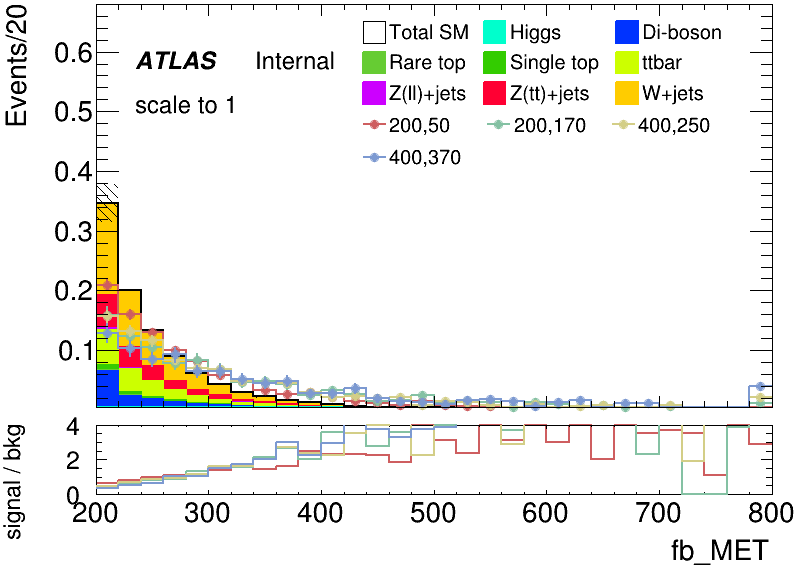
\includegraphics[width=\textwidth]{graphics/LH_met_sig/LH_fb_MET_norm.png}
    \end{minipage}
    \hfill
    \begin{minipage}{0.5\textwidth}
        \centering
        \setlength{\fboxsep}{0pt} % 边框与图片的距离
        \setlength{\fboxrule}{1pt} % 边框的粗细
        \fbox{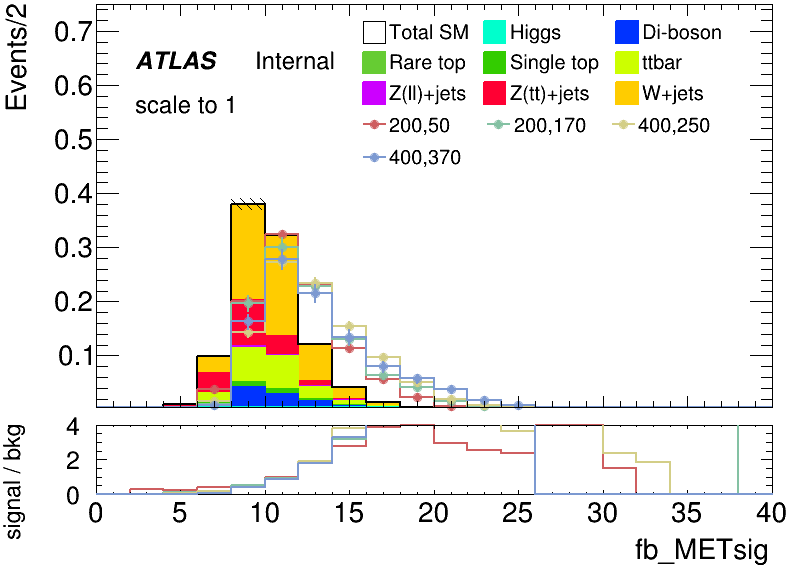
\includegraphics[width=\textwidth]{graphics/LH_met_sig/LH_fb_METsig_norm.png}}
    \end{minipage}
\end{frame}

\begin{frame}
\frametitle{kinematic distribution}
\framesubtitle{LH:num of obj}
%% 第一行
%    \begin{minipage}{0.2\textwidth}
%        \centering
%        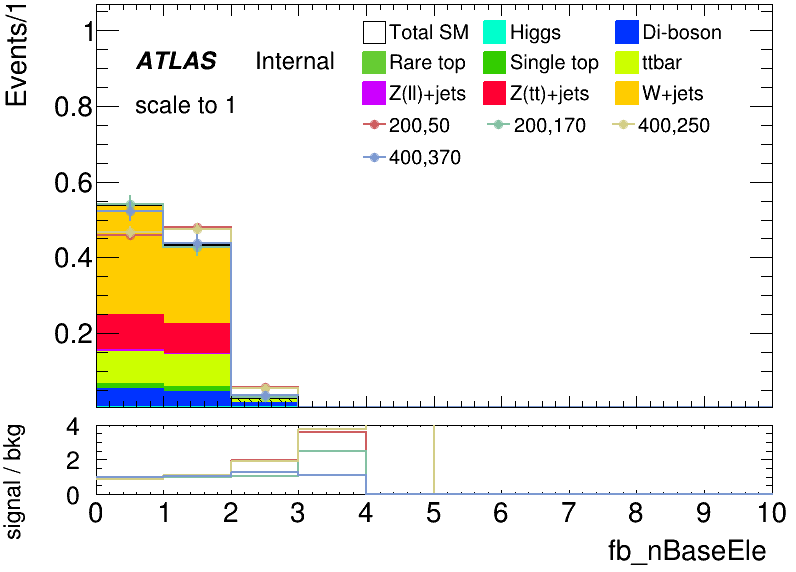
\includegraphics[width=\textwidth]{graphics/LH_met_sig/LH_fb_nBaseEle_norm.png}
%    \end{minipage}
%    \hfill
%    \begin{minipage}{0.2\textwidth}
%        \centering
%        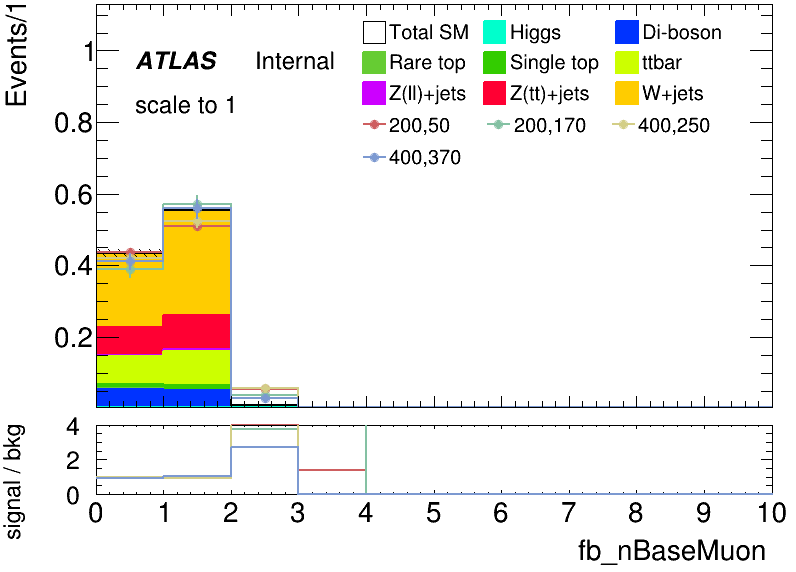
\includegraphics[width=\textwidth]{graphics/LH_met_sig/LH_fb_nBaseMuon_norm.png}
%    \end{minipage}
%    \hfill
%    \begin{minipage}{0.2\textwidth}
%        \centering
%        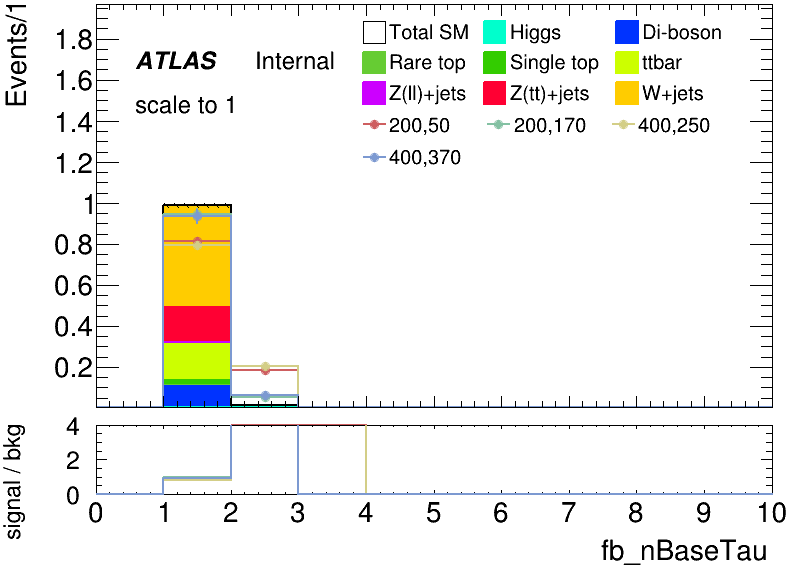
\includegraphics[width=\textwidth]{graphics/LH_met_sig/LH_fb_nBaseTau_norm.png}
%    \end{minipage}
%    \hfill
%    \begin{minipage}{0.2\textwidth}
%        \centering
%        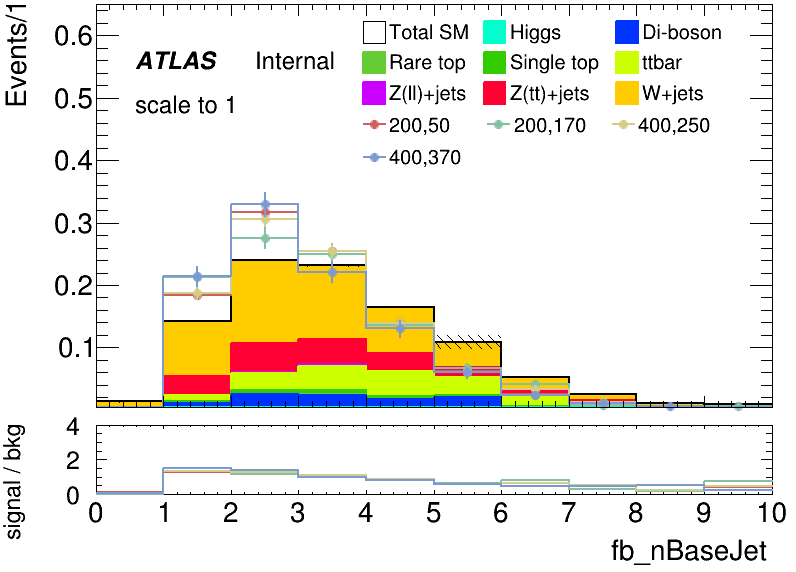
\includegraphics[width=\textwidth]{graphics/LH_met_sig/LH_fb_nBaseJet_norm.png}
%    \end{minipage}
%    \begin{minipage}{0.2\textwidth}
%        \centering
%        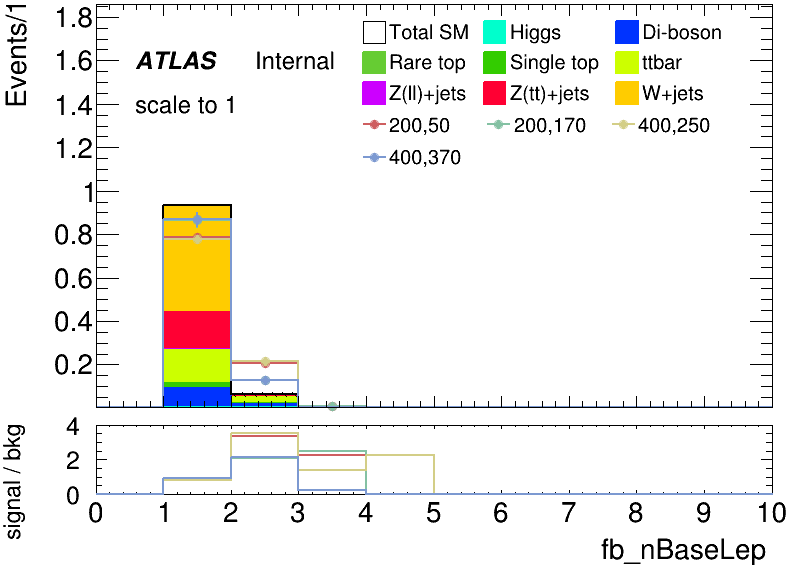
\includegraphics[width=\textwidth]{graphics/LH_met_sig/LH_fb_nBaseLep_norm.png}
%    \end{minipage}
%     
%    \vspace{0.5cm} % 图片之间的竖直间距

    % 第二行
    \begin{minipage}{0.32\textwidth}
        \centering
        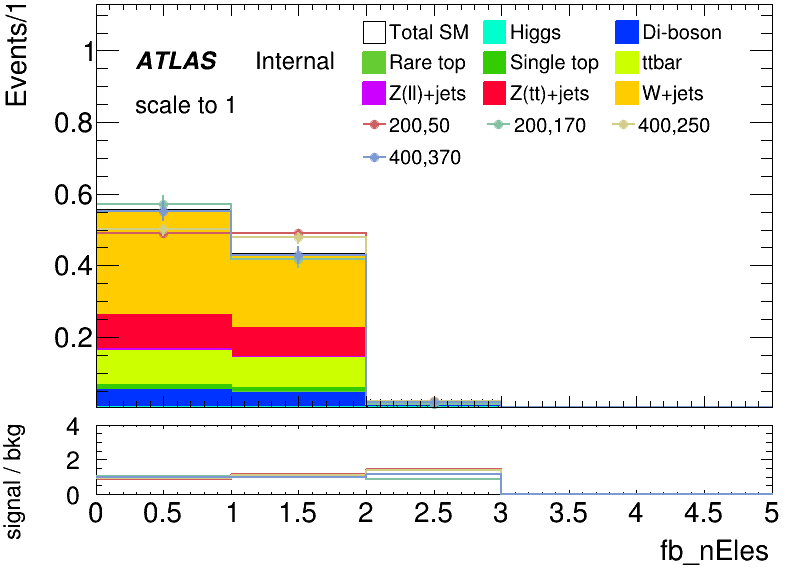
\includegraphics[width=\textwidth]{graphics/LH_met_sig/LH_fb_nEles_norm.png}
    \end{minipage}
    \hfill
    \begin{minipage}{0.32\textwidth}
        \centering
        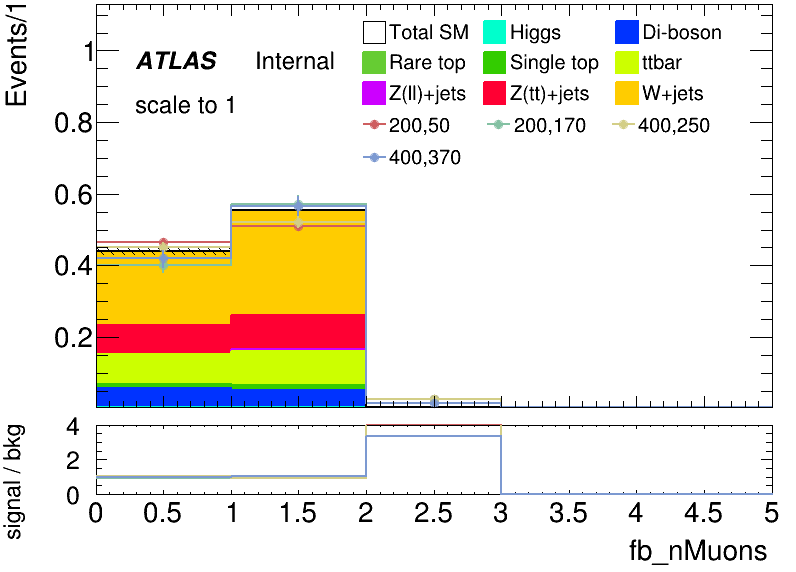
\includegraphics[width=\textwidth]{graphics/LH_met_sig/LH_fb_nMuons_norm.png}
    \end{minipage}
    \hfill
    \begin{minipage}{0.32\textwidth}
        \centering
        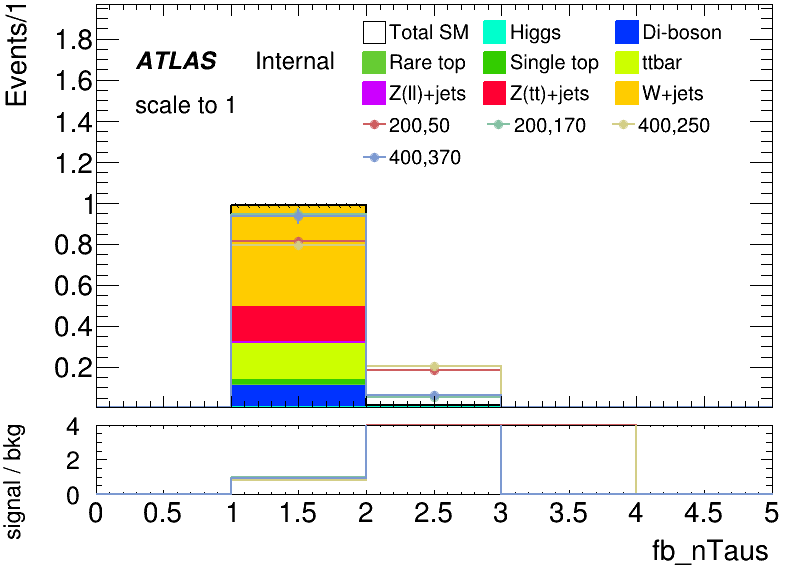
\includegraphics[width=\textwidth]{graphics/LH_met_sig/LH_fb_nTaus_norm.png}
    \end{minipage}
    \vspace{0.5cm}
    
    \begin{minipage}{0.32\textwidth}
        \centering
        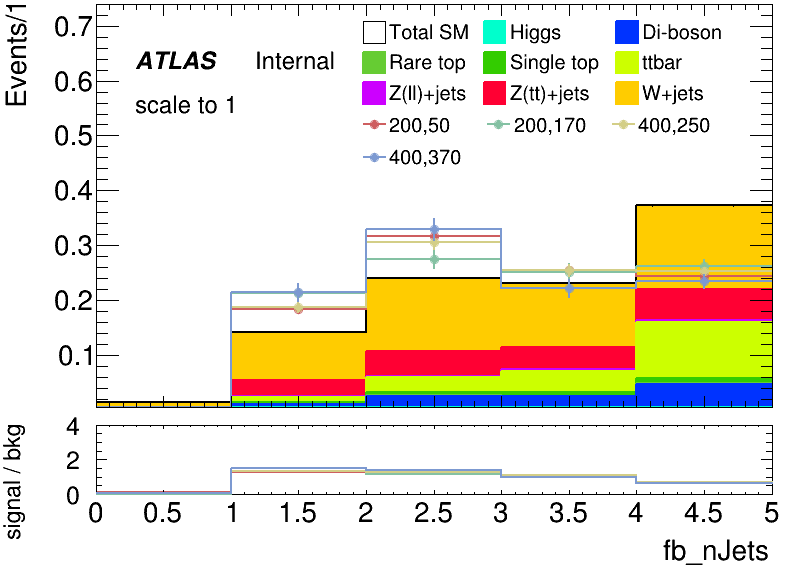
\includegraphics[width=\textwidth]{graphics/LH_met_sig/LH_fb_nJets_norm.png}
    \end{minipage}
    \begin{minipage}{0.32\textwidth}
        \centering
        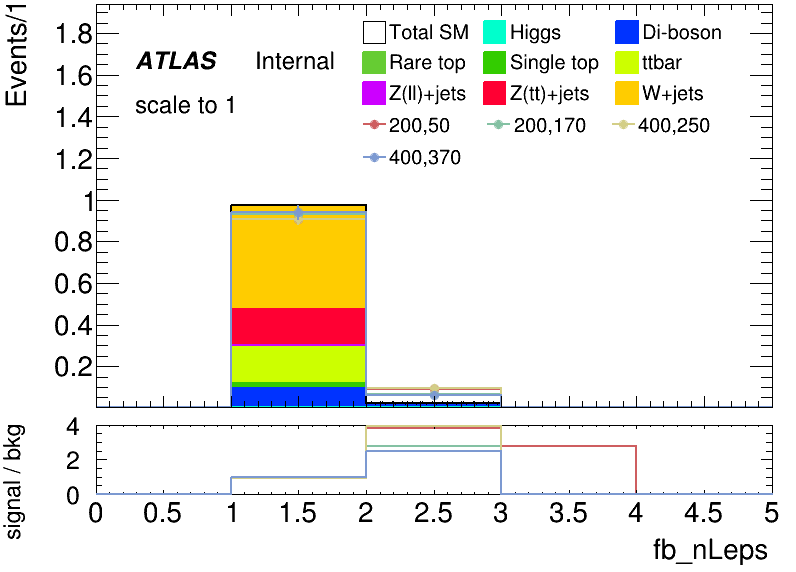
\includegraphics[width=\textwidth]{graphics/LH_met_sig/LH_fb_nLeps_norm.png}
    \end{minipage}
    \hfil
    \begin{minipage}{0.32\textwidth}
        \centering
        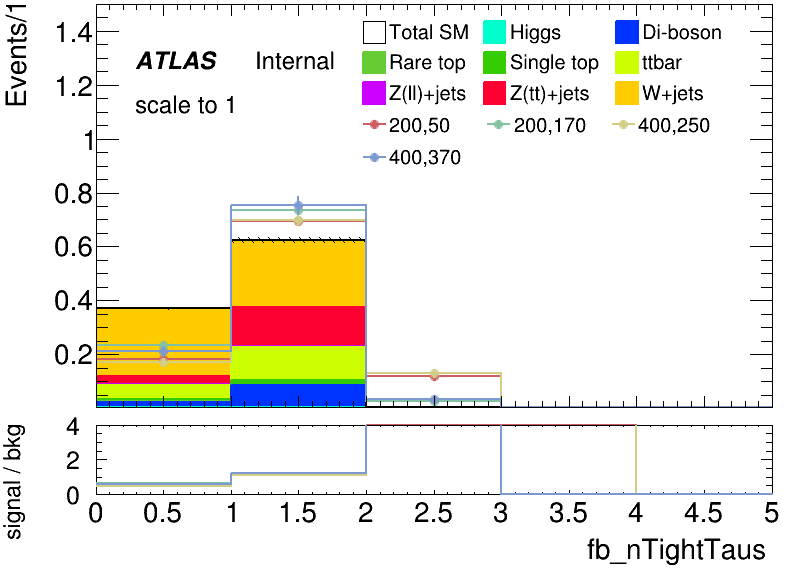
\includegraphics[width=\textwidth]{graphics/LH_met_sig/LH_fb_nTightTaus_norm.png}
    \end{minipage}
\end{frame}

\begin{frame}
	\frametitle{kinematic distribution}
	\framesubtitle{LH:num of obj}
%	    \begin{minipage}{0.25\textwidth}
%        \centering
%        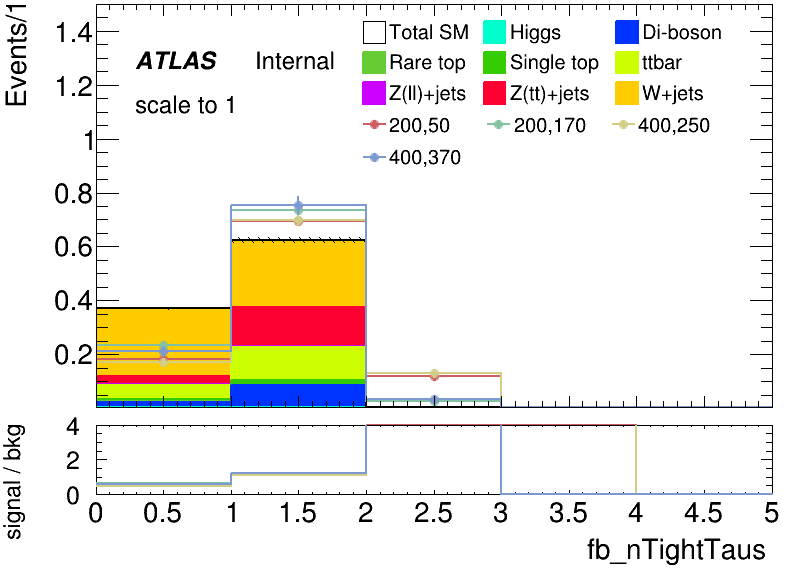
\includegraphics[width=\textwidth]{graphics/LH_met_sig/LH_fb_nTightTaus_norm.png}
%    \end{minipage}
%    \hfill
    \begin{minipage}{0.32\textwidth}
        \centering
        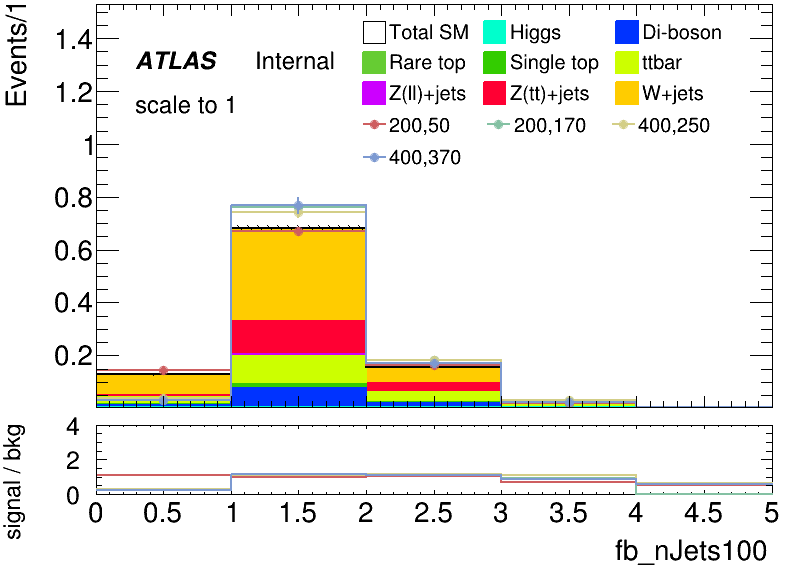
\includegraphics[width=\textwidth]{graphics/LH_met_sig/LH_fb_nJets100_norm.png}
    \end{minipage}
    \hfill
    \begin{minipage}{0.32\textwidth}
        \centering
        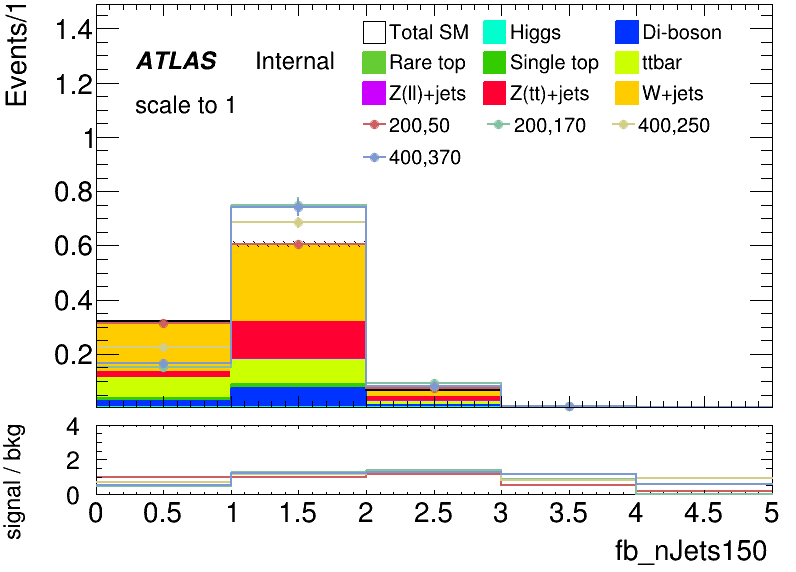
\includegraphics[width=\textwidth]{graphics/LH_met_sig/LH_fb_nJets150_norm.png}
    \end{minipage}
    \hfill
    \begin{minipage}{0.32\textwidth}
        \centering
        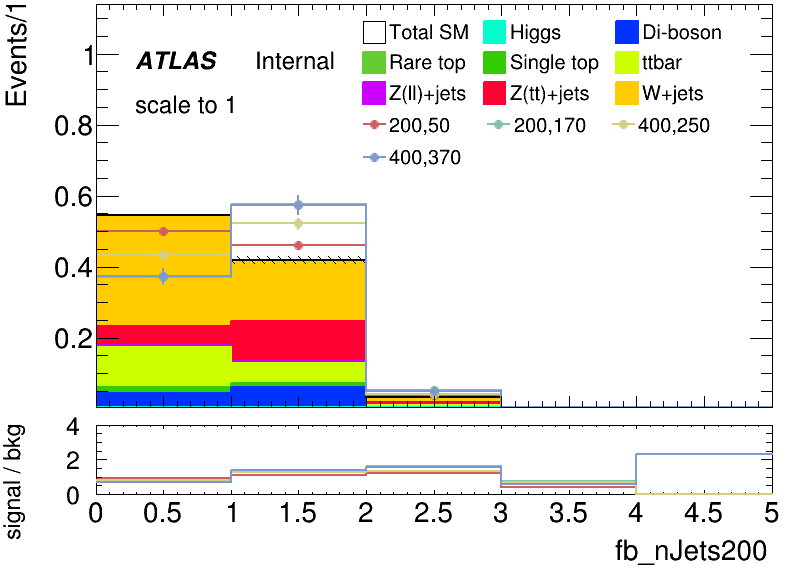
\includegraphics[width=\textwidth]{graphics/LH_met_sig/LH_fb_nJets200_norm.png}
    \end{minipage}
     
    \vspace{0.5cm} % 图片之间的竖直间距

    % 第二行
    \begin{minipage}{0.32\textwidth}
        \centering
        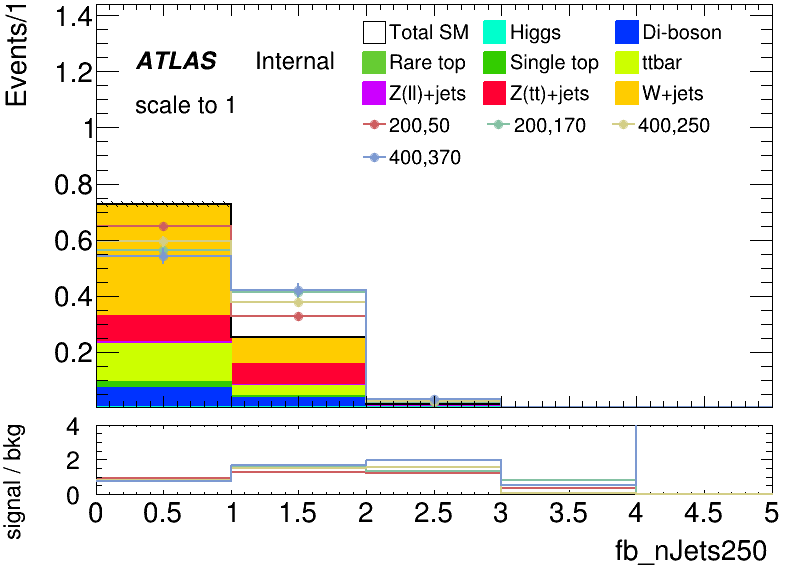
\includegraphics[width=\textwidth]{graphics/LH_met_sig/LH_fb_nJets250_norm.png}
    \end{minipage}
    \hfill
    \begin{minipage}{0.32\textwidth}
        \centering
        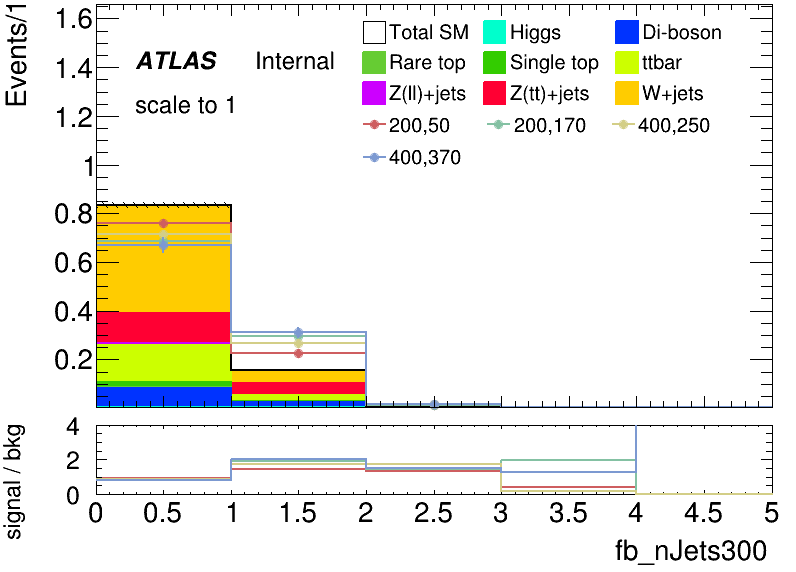
\includegraphics[width=\textwidth]{graphics/LH_met_sig/LH_fb_nJets300_norm.png}
    \end{minipage}
    \hfill
    \begin{minipage}{0.32\textwidth}
        \centering
        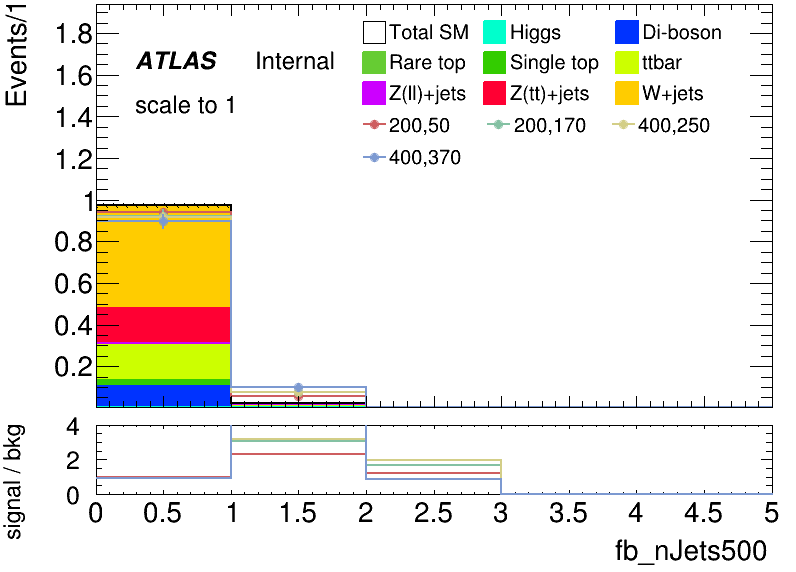
\includegraphics[width=\textwidth]{graphics/LH_met_sig/LH_fb_nJets500_norm.png}
    \end{minipage}
\end{frame}

\begin{frame}

	\frametitle{kinematic distribution}
	\framesubtitle{LH:$m_{inv}$}
    \begin{minipage}{0.32\textwidth}
        \centering
        \setlength{\fboxsep}{0pt} % 边框与图片的距离
        \setlength{\fboxrule}{1pt} % 边框的粗细
        \fbox{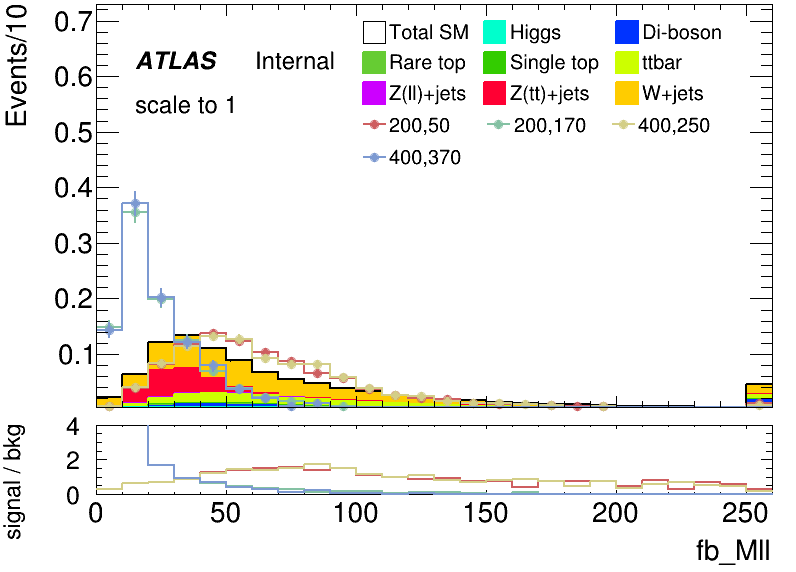
\includegraphics[width=\textwidth]{graphics/LH_met_sig/LH_fb_Mll_norm.png}}
    \end{minipage}
    \hfill
    \begin{minipage}{0.32\textwidth}
        \centering
        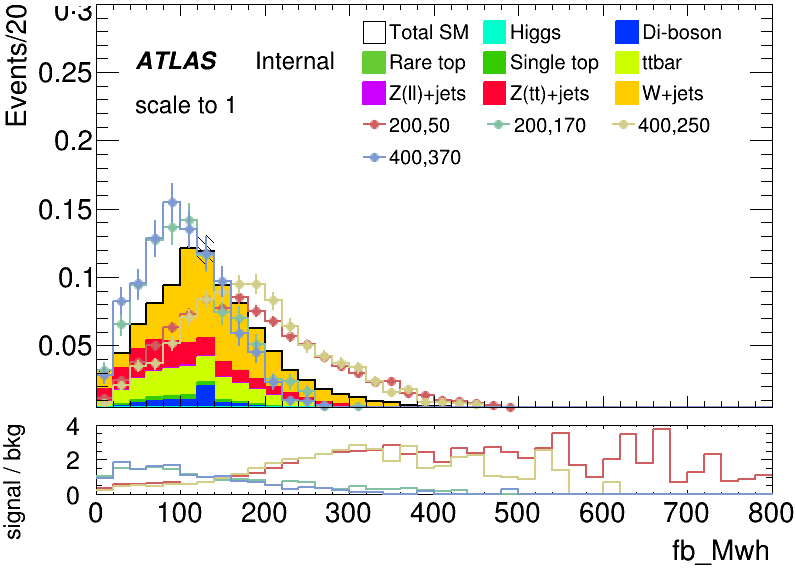
\includegraphics[width=\textwidth]{graphics/LH_met_sig/LH_fb_Mwh_norm.png}
    \end{minipage}
    \hfill
    \begin{minipage}{0.32\textwidth}
        \centering
        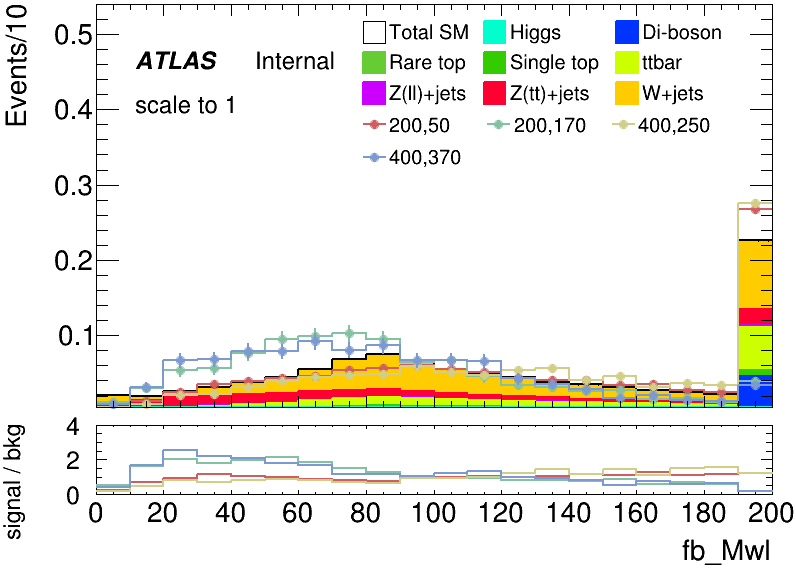
\includegraphics[width=\textwidth]{graphics/LH_met_sig/LH_fb_Mwl_norm.png}
    \end{minipage}	
notice:Mll is the invariant between tau1 and tau2, Mwh is the invariant between tau1 and MET, Mwl is the invariant between tau2 and MET  
\end{frame}

\begin{frame}
	\frametitle{kinematic distribution}
	\framesubtitle{LH:transverse mass}
	    \begin{minipage}{0.25\textwidth}
        \centering
        \setlength{\fboxsep}{0pt} % 边框与图片的距离
        \setlength{\fboxrule}{1pt} % 边框的粗细
        \fbox{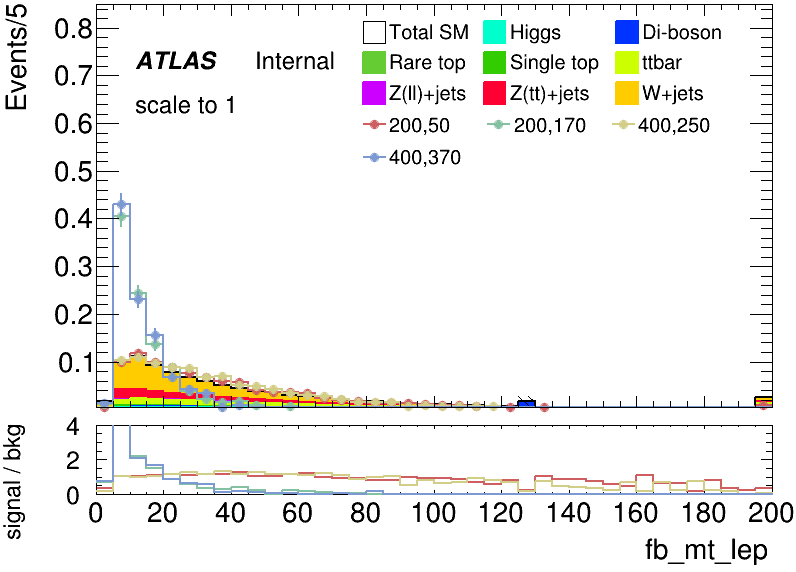
\includegraphics[width=\textwidth]{graphics/LH_met_sig/LH_fb_mt_lep_norm.png}}
    \end{minipage}
    \hfill
    \begin{minipage}{0.25\textwidth}
        \centering
        \setlength{\fboxsep}{0pt} % 边框与图片的距离
        \setlength{\fboxrule}{1pt} % 边框的粗细
        \fbox{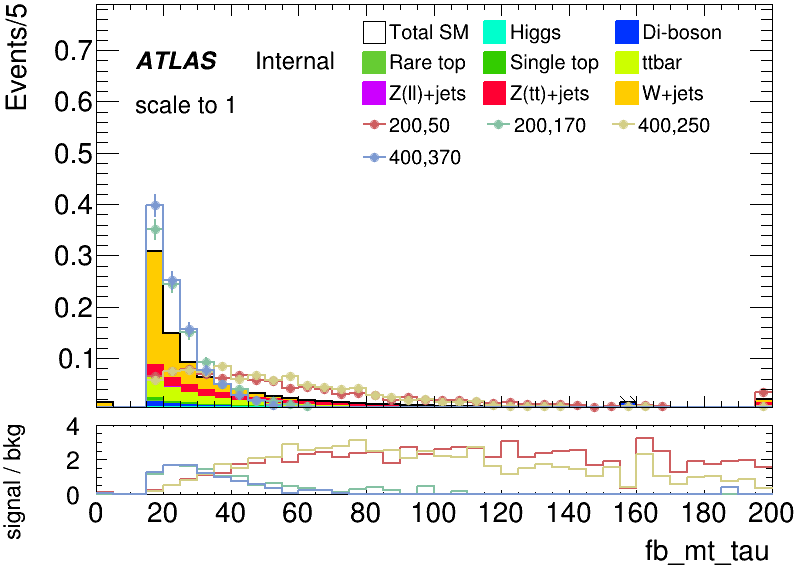
\includegraphics[width=\textwidth]{graphics/LH_met_sig/LH_fb_mt_tau_norm.png}}
    \end{minipage}
    \hfill
    \begin{minipage}{0.25\textwidth}
        \centering
        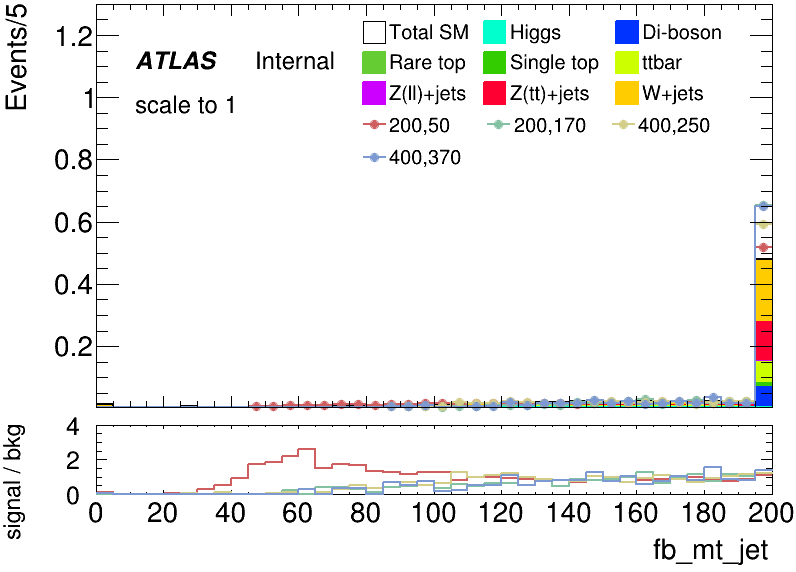
\includegraphics[width=\textwidth]{graphics/LH_met_sig/LH_fb_mt_jet_norm.png}
    \end{minipage}
    \hfill
    \begin{minipage}{0.25\textwidth}
        \centering
        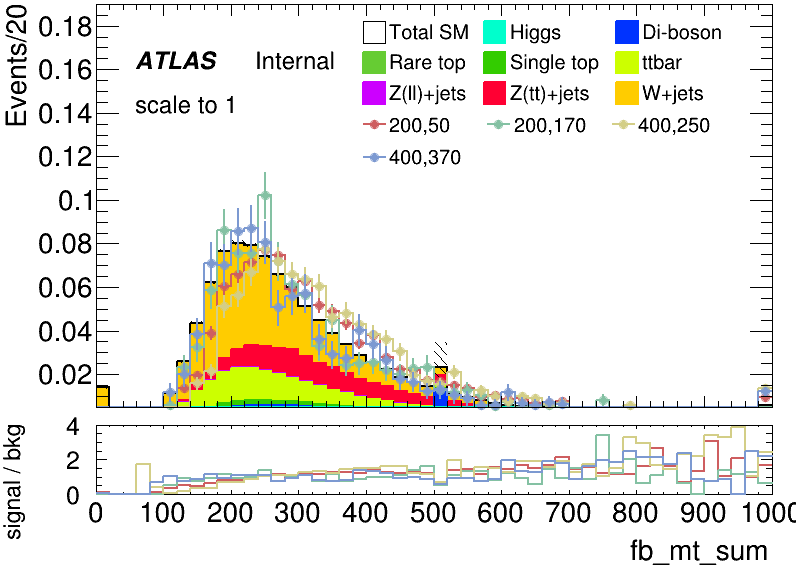
\includegraphics[width=\textwidth]{graphics/LH_met_sig/LH_fb_mt_sum_norm.png}
    \end{minipage}
\end{frame}
\begin{frame}
\frametitle{kinematic distribution}
\framesubtitle{LH:MT2}
    \begin{minipage}{0.32\textwidth}
        \centering
        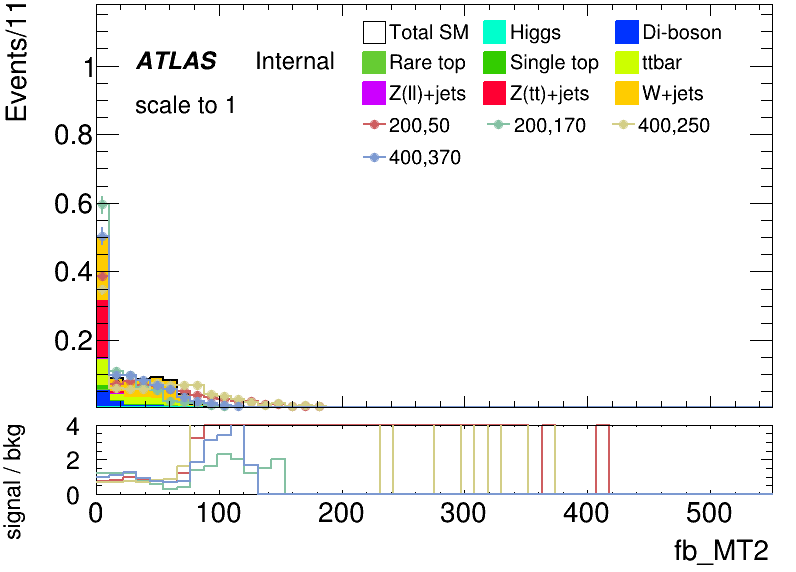
\includegraphics[width=\textwidth]{graphics/LH_met_sig/LH_fb_MT2_norm.png}
    \end{minipage}
    \hfill
    \begin{minipage}{0.32\textwidth}
        \centering
        \setlength{\fboxsep}{0pt} % 边框与图片的距离
        \setlength{\fboxrule}{1pt} % 边框的粗细
        \fbox{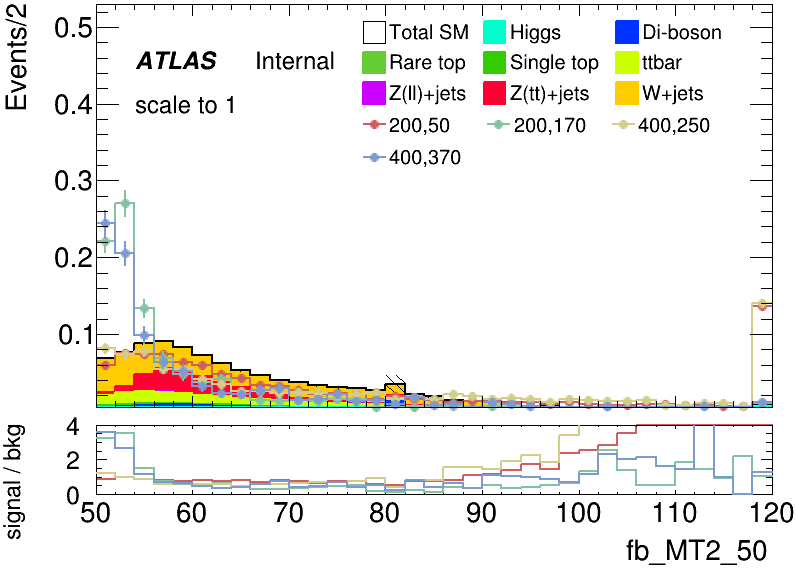
\includegraphics[width=\textwidth]{graphics/LH_met_sig/LH_fb_MT2_50_norm.png}}
    \end{minipage}
    \hfill
    \begin{minipage}{0.32\textwidth}
        \centering
        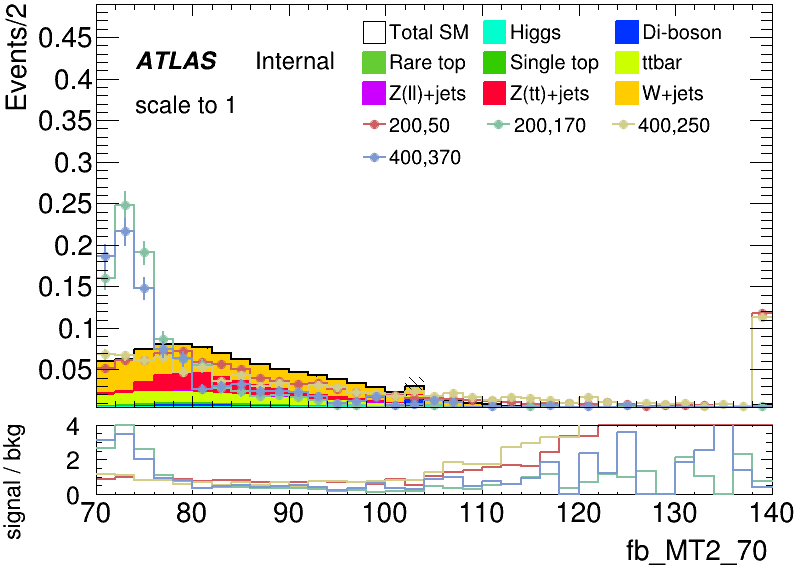
\includegraphics[width=\textwidth]{graphics/LH_met_sig/LH_fb_MT2_70_norm.png}
    \end{minipage}
    
    \vspace{0.5cm}

    \begin{minipage}{0.32\textwidth}
        \centering
        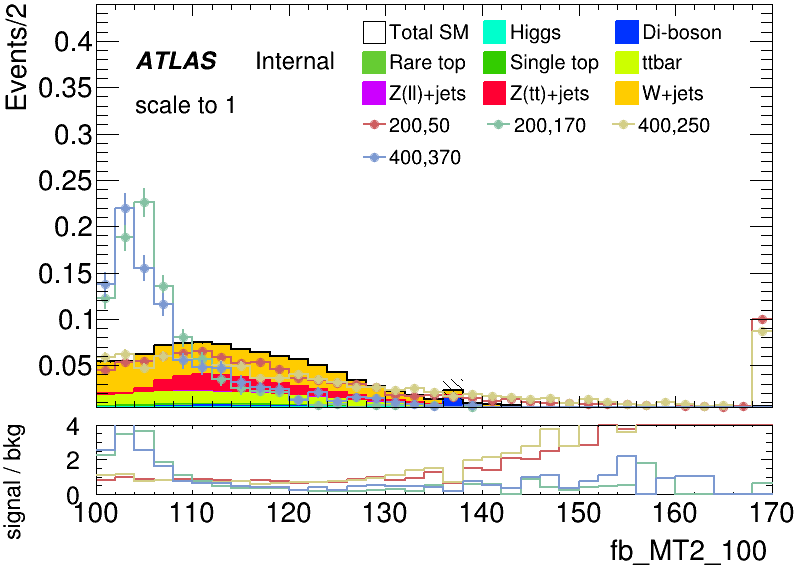
\includegraphics[width=\textwidth]{graphics/LH_met_sig/LH_fb_MT2_100_norm.png}
    \end{minipage}
    \hfill
    \begin{minipage}{0.32\textwidth}
        \centering
        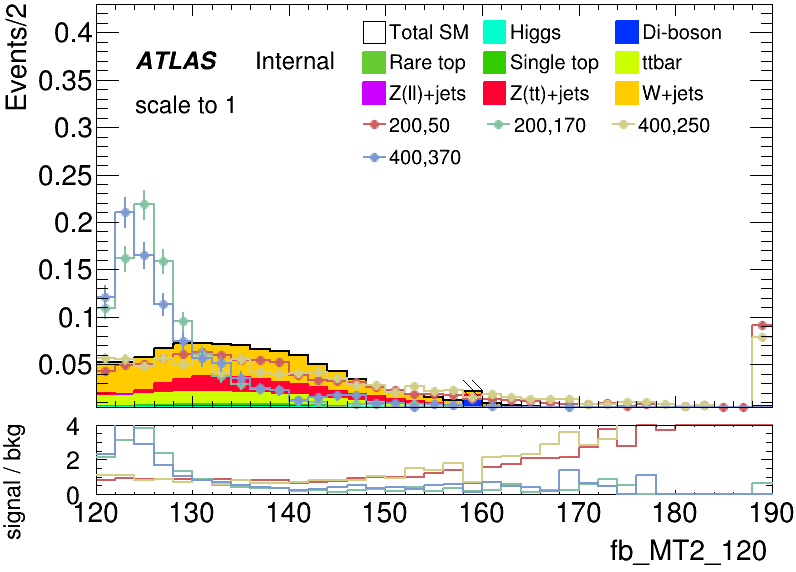
\includegraphics[width=\textwidth]{graphics/LH_met_sig/LH_fb_MT2_120_norm.png}
    \end{minipage}
    \hfill
    \begin{minipage}{0.32\textwidth}
        \centering
        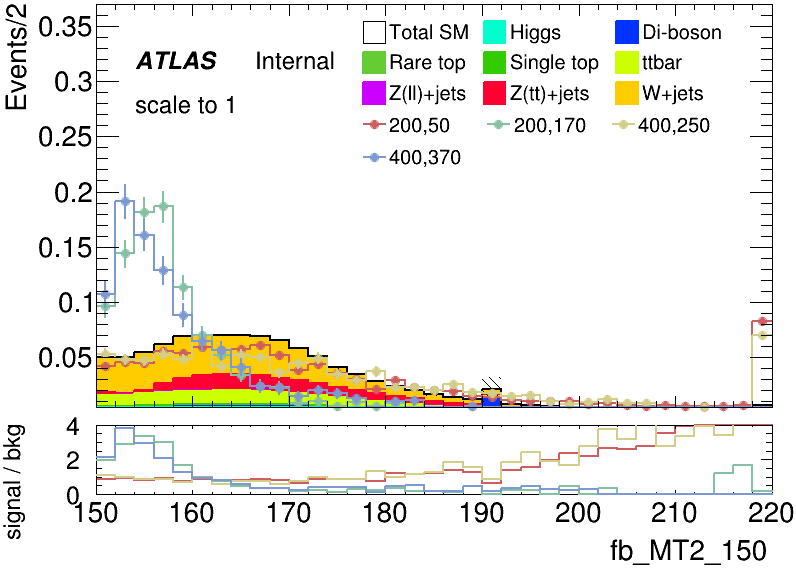
\includegraphics[width=\textwidth]{graphics/LH_met_sig/LH_fb_MT2_150_norm.png}
    \end{minipage}
\end{frame}

%\begin{frame}
%	\frametitle{kinematic distribution}
%	\framesubtitle{LH:ratio}
%    \begin{minipage}{0.32\textwidth}
%        \centering
%        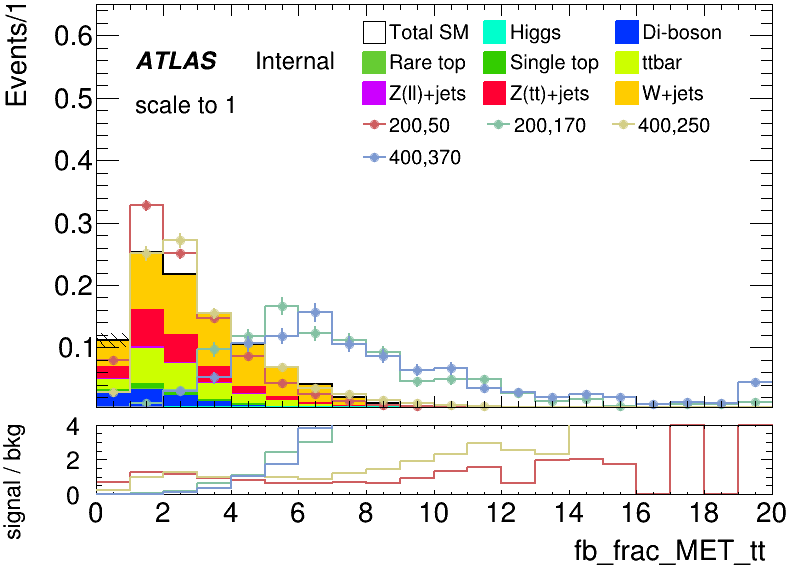
\includegraphics[width=\textwidth]{graphics/LH_met_sig/LH_fb_frac_MET_tt_norm.png}
%    \end{minipage}
%    \hfill
%    \begin{minipage}{0.32\textwidth}
%        \centering
%        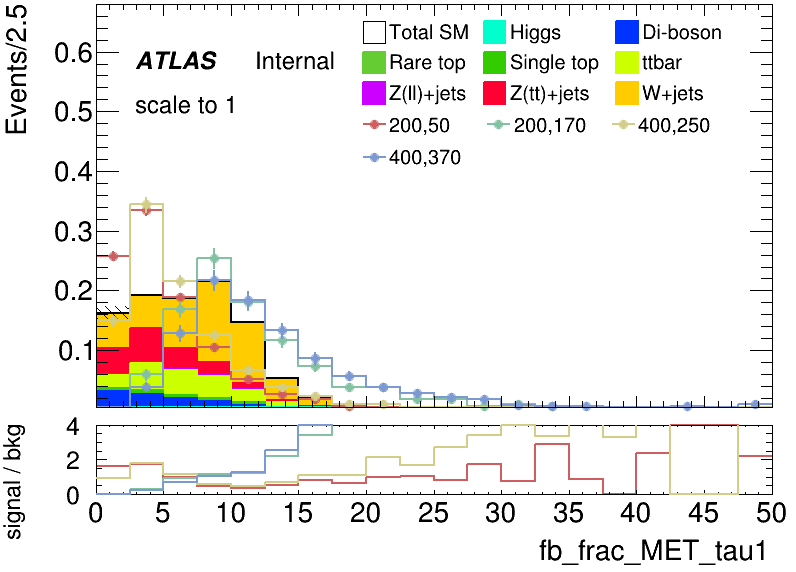
\includegraphics[width=\textwidth]{graphics/LH_met_sig/LH_fb_frac_MET_tau1_norm.png}
%    \end{minipage}
%    \hfill
%    \begin{minipage}{0.32\textwidth}
%        \centering
%        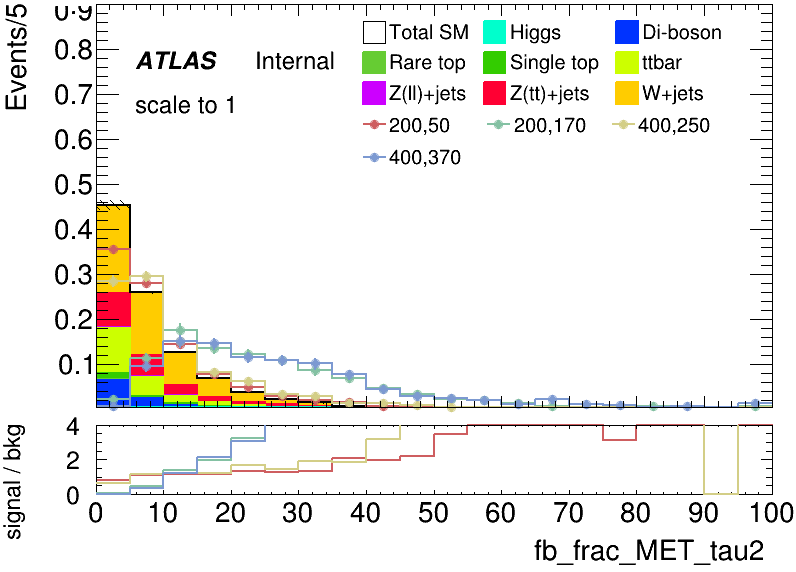
\includegraphics[width=\textwidth]{graphics/LH_met_sig/LH_fb_frac_MET_tau2_norm.png}
%    \end{minipage}
%    
%    \vspace{0.5cm}
%
%    \begin{minipage}{0.32\textwidth}
%        \centering
%        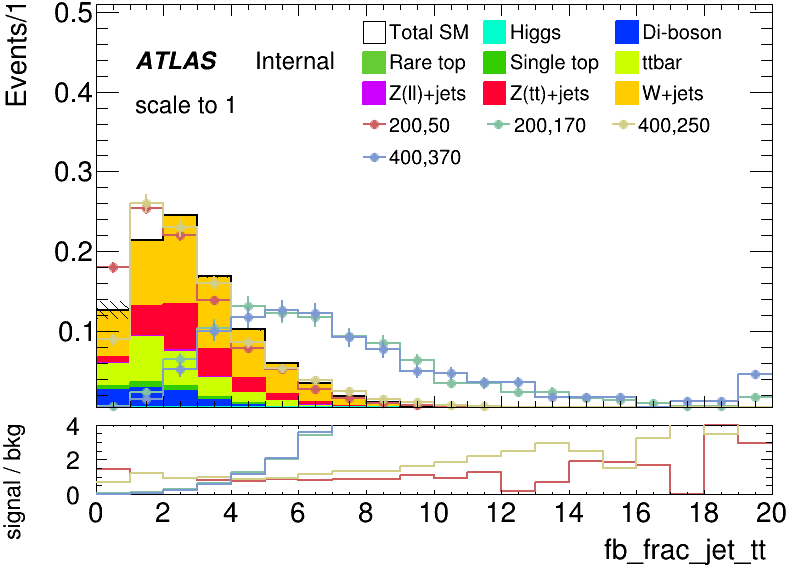
\includegraphics[width=\textwidth]{graphics/LH_met_sig/LH_fb_frac_jet_tt_norm.png}
%    \end{minipage}
%    \hfill
%    \begin{minipage}{0.32\textwidth}
%        \centering
%        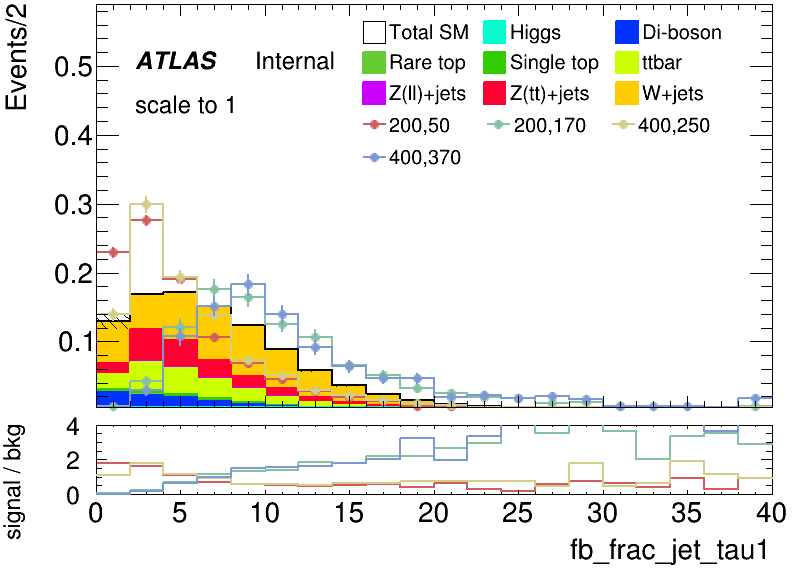
\includegraphics[width=\textwidth]{graphics/LH_met_sig/LH_fb_frac_jet_tau1_norm.png}
%    \end{minipage}
%    \hfill
%    \begin{minipage}{0.32\textwidth}
%        \centering
%        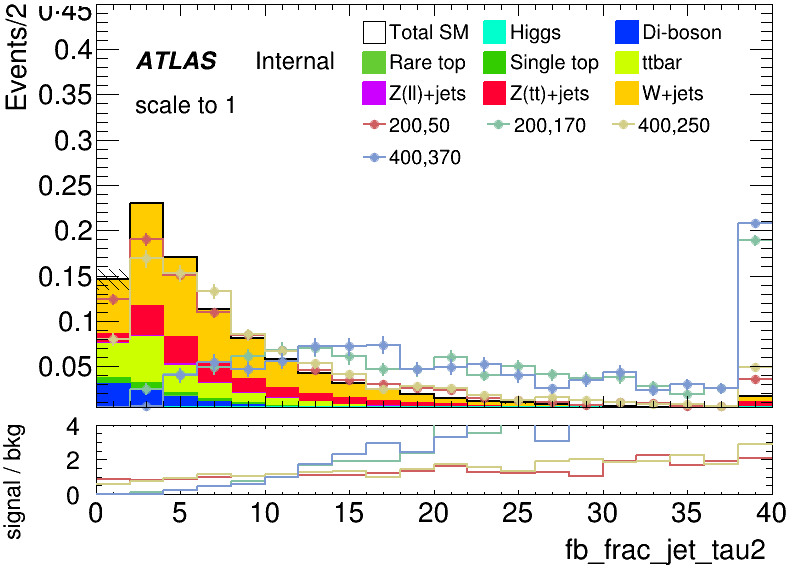
\includegraphics[width=\textwidth]{graphics/LH_met_sig/LH_fb_frac_jet_tau2_norm.png}
%    \end{minipage}	
%\end{frame}

\begin{frame}
  \frametitle{kinematic distribution}
  \framesubtitle{LH:$\Delta R$}
    \begin{minipage}{0.32\textwidth}
        \centering
        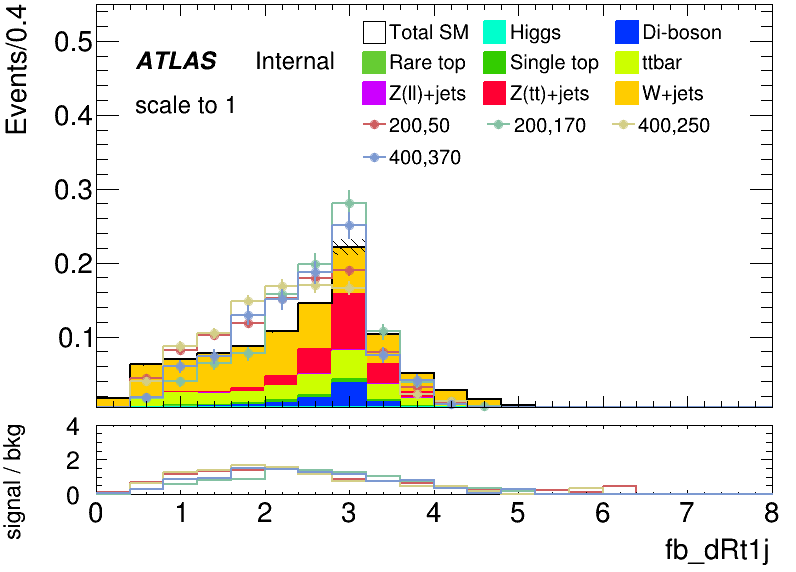
\includegraphics[width=\textwidth]{graphics/LH_met_sig/LH_fb_dRt1j_norm.png}
    \end{minipage}
    \hfill
    \begin{minipage}{0.32\textwidth}
        \centering
        \setlength{\fboxsep}{0pt} % 边框与图片的距离
        \setlength{\fboxrule}{1pt} % 边框的粗细
        \fbox{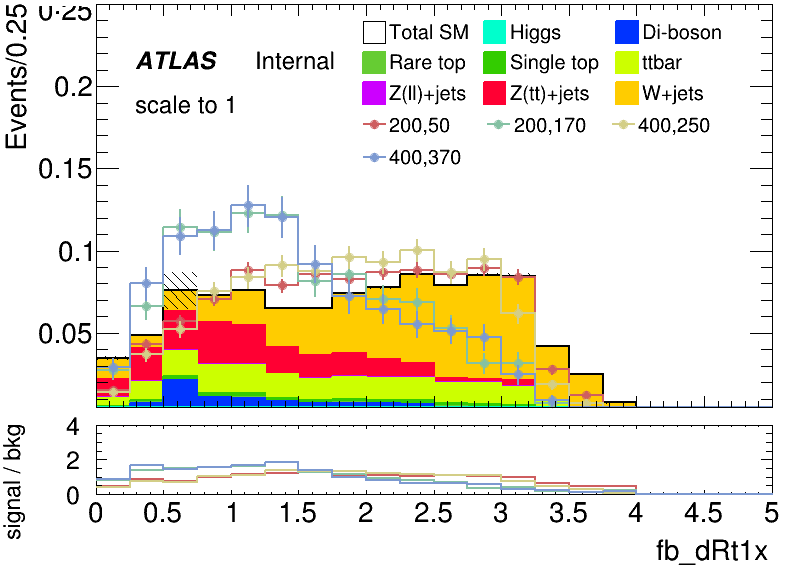
\includegraphics[width=\textwidth]{graphics/LH_met_sig/LH_fb_dRt1x_norm.png}}
    \end{minipage}
    \hfill
    \begin{minipage}{0.32\textwidth}
        \centering
        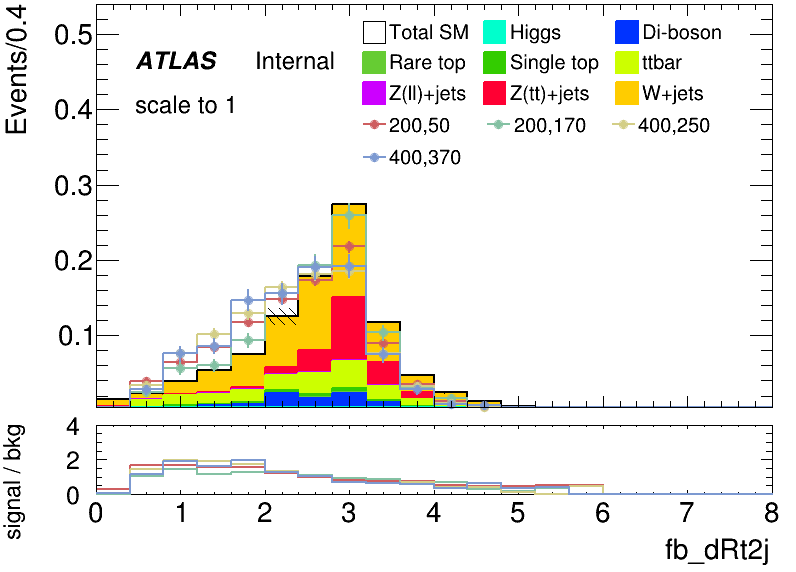
\includegraphics[width=\textwidth]{graphics/LH_met_sig/LH_fb_dRt2j_norm.png}
    \end{minipage}
    
    \vspace{0.5cm} % 图片之间的竖直间距

    % 第二行
    \begin{minipage}{0.32\textwidth}
        \centering
        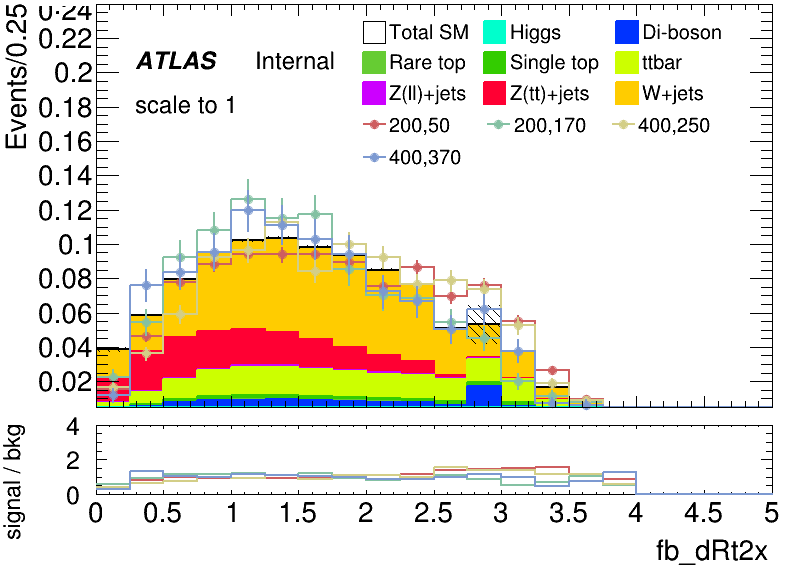
\includegraphics[width=\textwidth]{graphics/LH_met_sig/LH_fb_dRt2x_norm.png}
    \end{minipage}
    \hfill
    \begin{minipage}{0.32\textwidth}
        \centering
        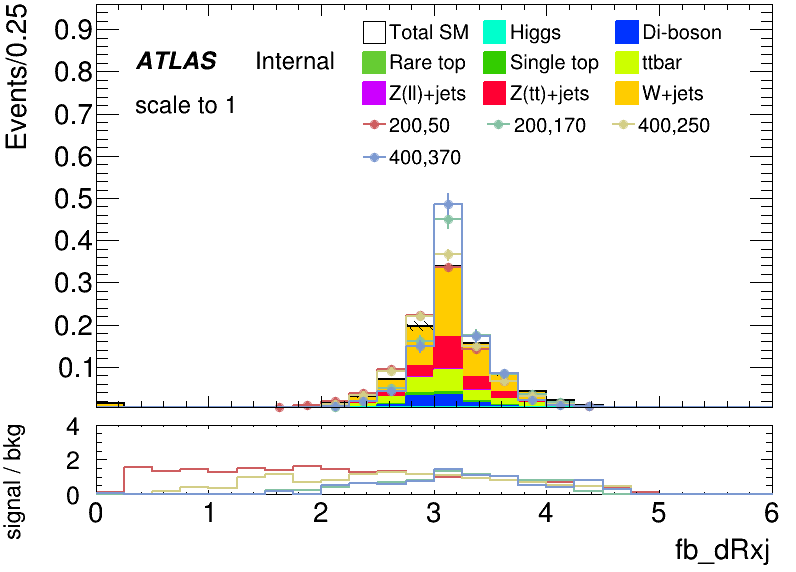
\includegraphics[width=\textwidth]{graphics/LH_met_sig/LH_fb_dRxj_norm.png}
    \end{minipage}
    \hfill
    \begin{minipage}{0.32\textwidth}
        \centering
        \setlength{\fboxsep}{0pt} % 边框与图片的距离
        \setlength{\fboxrule}{1pt} % 边框的粗细
        \fbox{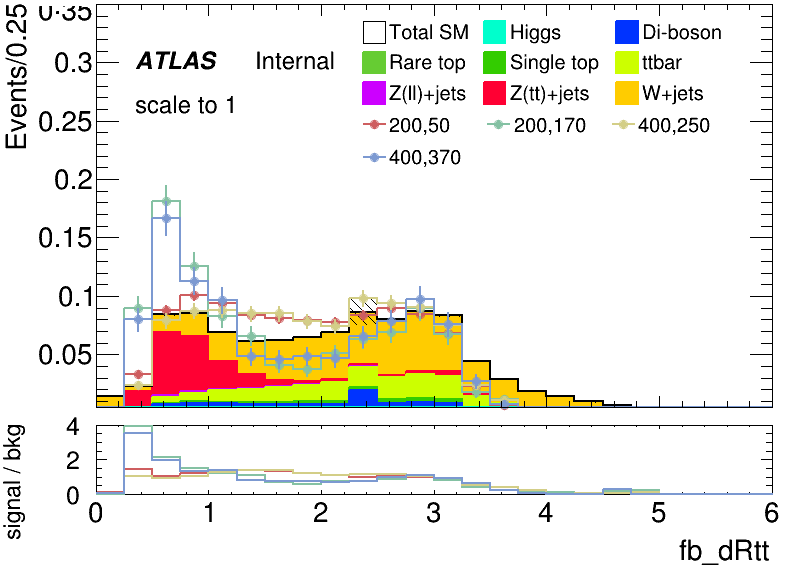
\includegraphics[width=\textwidth]{graphics/LH_met_sig/LH_fb_dRtt_norm.png}}
    \end{minipage}
    notice: t1 is leading tau, t2 is leading lep, j is leading jet, x is MET.
\end{frame}

\begin{frame}
  \frametitle{kinematic distribution}
  \framesubtitle{LH:$\Delta\phi$}
    \begin{minipage}{0.32\textwidth}
        \centering
        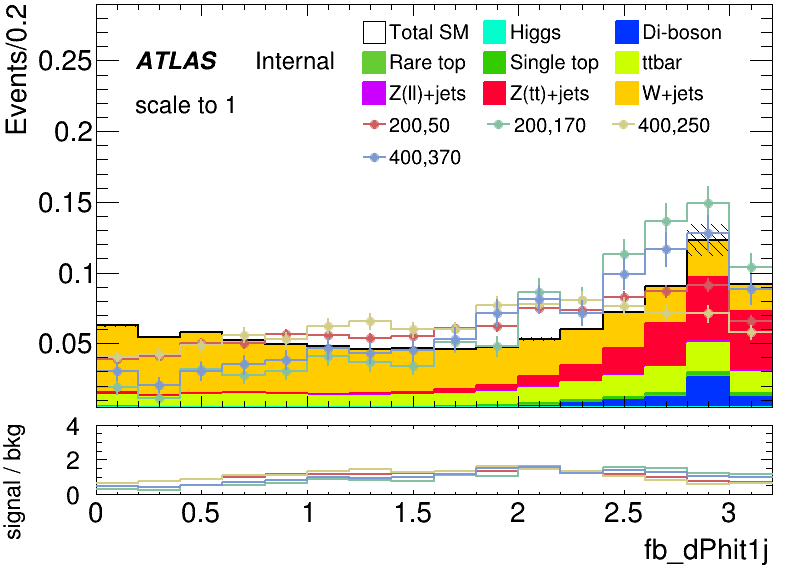
\includegraphics[width=\textwidth]{graphics/LH_met_sig/LH_fb_dPhit1j_norm.png}
    \end{minipage}
    \hfill
    \begin{minipage}{0.32\textwidth}
        \centering
        \includegraphics[width=\textwidth]{graphics/LH_met_sig/LH_fb_dPhit1x_norm.png}
    \end{minipage}
    \hfill
    \begin{minipage}{0.32\textwidth}
        \centering
        \includegraphics[width=\textwidth]{graphics/LH_met_sig/LH_fb_dPhit2j_norm.png}
    \end{minipage}
    
    \vspace{0.5cm} % 图片之间的竖直间距

    % 第二行
    \begin{minipage}{0.32\textwidth}
        \centering
        \includegraphics[width=\textwidth]{graphics/LH_met_sig/LH_fb_dPhit2x_norm.png}
    \end{minipage}
    \hfill
    \begin{minipage}{0.32\textwidth}
        \centering
        \includegraphics[width=\textwidth]{graphics/LH_met_sig/LH_fb_dPhixj_norm.png}
    \end{minipage}
    \hfill
    \begin{minipage}{0.32\textwidth}
        \centering
        \includegraphics[width=\textwidth]{graphics/LH_met_sig/LH_fb_dPhitt_norm.png}
    \end{minipage}
    notice: t1 is leading tau, t2 is leading lep, j is leading jet, x is MET.
\end{frame}

\subsection{HH kinematic distribution}
\begin{frame}
	\frametitle{kinematic distribution}
	\framesubtitle{HH:$p_T$}
For sig/bkg, both bkg and signal distribution are normalized to 1. Kinematic variables with better separation power are marked with black box.

% 第一行
    \begin{minipage}{0.32\textwidth}
        \centering
        \includegraphics[width=\textwidth]{graphics/HH_met_sig/HH_fb_pt_jet_norm.png}
    \end{minipage}
    \hfill
    \begin{minipage}{0.32\textwidth}
        \centering
        \includegraphics[width=\textwidth]{graphics/HH_met_sig/HH_fb_pt_lep_norm.png}
    \end{minipage}
    \hfill
    \begin{minipage}{0.32\textwidth}
        \centering
        \includegraphics[width=\textwidth]{graphics/HH_met_sig/HH_fb_pt_tau_norm.png}
    \end{minipage}
    
    \vspace{0.5cm} % 图片之间的竖直间距
    
    notice: t1 is leading tau, t2 is leading lep, j is leading jet, x is MET.
\end{frame}

\begin{frame}
  \frametitle{kinematic distribution}
  \framesubtitle{HH:MET}
    \begin{minipage}{0.5\textwidth}
        \centering
        \includegraphics[width=\textwidth]{graphics/HH_met_sig/HH_fb_MET_norm.png}
    \end{minipage}
    \hfill
    \begin{minipage}{0.5\textwidth}
        \centering
        \includegraphics[width=\textwidth]{graphics/HH_met_sig/HH_fb_METsig_norm.png}
    \end{minipage}
\end{frame}

\begin{frame}
\frametitle{kinematic distribution}
\framesubtitle{HH:num of obj}
%% 第一行
%    \begin{minipage}{0.2\textwidth}
%        \centering
%        \includegraphics[width=\textwidth]{graphics/HH_met_sig/HH_fb_nBaseEle_norm.png}
%    \end{minipage}
%    \hfill
%    \begin{minipage}{0.2\textwidth}
%        \centering
%        \includegraphics[width=\textwidth]{graphics/HH_met_sig/HH_fb_nBaseMuon_norm.png}
%    \end{minipage}
%    \hfill
%    \begin{minipage}{0.2\textwidth}
%        \centering
%        \includegraphics[width=\textwidth]{graphics/HH_met_sig/HH_fb_nBaseTau_norm.png}
%    \end{minipage}
%    \hfill
%    \begin{minipage}{0.2\textwidth}
%        \centering
%        \includegraphics[width=\textwidth]{graphics/HH_met_sig/HH_fb_nBaseJet_norm.png}
%    \end{minipage}
%    \begin{minipage}{0.2\textwidth}
%        \centering
%        \includegraphics[width=\textwidth]{graphics/HH_met_sig/HH_fb_nBaseLep_norm.png}
%    \end{minipage}
%     
%    \vspace{0.5cm} % 图片之间的竖直间距

    % 第二行
    \begin{minipage}{0.32\textwidth}
        \centering
        \includegraphics[width=\textwidth]{graphics/HH_met_sig/HH_fb_nEles_norm.png}
    \end{minipage}
    \hfill
    \begin{minipage}{0.32\textwidth}
        \centering
        \includegraphics[width=\textwidth]{graphics/HH_met_sig/HH_fb_nMuons_norm.png}
    \end{minipage}
    \hfill
    \begin{minipage}{0.32\textwidth}
        \centering
        \includegraphics[width=\textwidth]{graphics/HH_met_sig/HH_fb_nTaus_norm.png}
    \end{minipage}
    \vspace{0.5cm}
    
    \begin{minipage}{0.32\textwidth}
        \centering
        \includegraphics[width=\textwidth]{graphics/HH_met_sig/HH_fb_nJets_norm.png}
    \end{minipage}
    \begin{minipage}{0.32\textwidth}
        \centering
        \includegraphics[width=\textwidth]{graphics/HH_met_sig/HH_fb_nLeps_norm.png}
    \end{minipage}
    \hfil
    \begin{minipage}{0.32\textwidth}
        \centering
        \includegraphics[width=\textwidth]{graphics/HH_met_sig/HH_fb_nTightTaus_norm.png}
    \end{minipage}
\end{frame}

\begin{frame}
	\frametitle{kinematic distribution}
	\framesubtitle{HH:num of obj}
%	    \begin{minipage}{0.25\textwidth}
%        \centering
%        \includegraphics[width=\textwidth]{graphics/HH_met_sig/HH_fb_nTightTaus_norm.png}
%    \end{minipage}
%    \hfill
    \begin{minipage}{0.32\textwidth}
        \centering
        \includegraphics[width=\textwidth]{graphics/HH_met_sig/HH_fb_nJets100_norm.png}
    \end{minipage}
    \hfill
    \begin{minipage}{0.32\textwidth}
        \centering
        \includegraphics[width=\textwidth]{graphics/HH_met_sig/HH_fb_nJets150_norm.png}
    \end{minipage}
    \hfill
    \begin{minipage}{0.32\textwidth}
        \centering
        \includegraphics[width=\textwidth]{graphics/HH_met_sig/HH_fb_nJets200_norm.png}
    \end{minipage}
     
    \vspace{0.5cm} % 图片之间的竖直间距

    % 第二行
    \begin{minipage}{0.32\textwidth}
        \centering
        \includegraphics[width=\textwidth]{graphics/HH_met_sig/HH_fb_nJets250_norm.png}
    \end{minipage}
    \hfill
    \begin{minipage}{0.32\textwidth}
        \centering
        \includegraphics[width=\textwidth]{graphics/HH_met_sig/HH_fb_nJets300_norm.png}
    \end{minipage}
    \hfill
    \begin{minipage}{0.32\textwidth}
        \centering
        \includegraphics[width=\textwidth]{graphics/HH_met_sig/HH_fb_nJets500_norm.png}
    \end{minipage}
\end{frame}

\begin{frame}

	\frametitle{kinematic distribution}
	\framesubtitle{HH:$m_{inv}$}
    \begin{minipage}{0.32\textwidth}
        \centering
        \setlength{\fboxsep}{0pt} % 边框与图片的距离
        \setlength{\fboxrule}{1pt} % 边框的粗细
        \fbox{\includegraphics[width=\textwidth]{graphics/HH_met_sig/HH_fb_Mll_norm.png}}
    \end{minipage}
    \hfill
    \begin{minipage}{0.32\textwidth}
        \centering
        \includegraphics[width=\textwidth]{graphics/HH_met_sig/HH_fb_Mwh_norm.png}
    \end{minipage}
    \hfill
    \begin{minipage}{0.32\textwidth}
        \centering
        \includegraphics[width=\textwidth]{graphics/HH_met_sig/HH_fb_Mwl_norm.png}
    \end{minipage}	
notice:Mll is the invariant between tau1 and tau2, Mwh is the invariant between tau1 and MET, Mwl is the invariant between tau2 and MET  
\end{frame}

\begin{frame}
	\frametitle{kinematic distribution}
	\framesubtitle{HH:transverse mass}
	    \begin{minipage}{0.25\textwidth}
        \centering
        \includegraphics[width=\textwidth]{graphics/HH_met_sig/HH_fb_mt_lep_norm.png}
    \end{minipage}
    \hfill
    \begin{minipage}{0.25\textwidth}
        \centering
        \includegraphics[width=\textwidth]{graphics/HH_met_sig/HH_fb_mt_tau_norm.png}
    \end{minipage}
    \hfill
    \begin{minipage}{0.25\textwidth}
        \centering
        \includegraphics[width=\textwidth]{graphics/HH_met_sig/HH_fb_mt_jet_norm.png}
    \end{minipage}
    \hfill
    \begin{minipage}{0.25\textwidth}
        \centering
        \includegraphics[width=\textwidth]{graphics/HH_met_sig/HH_fb_mt_sum_norm.png}
    \end{minipage}
\end{frame}
\begin{frame}
\frametitle{kinematic distribution}
\framesubtitle{HH:MT2}
    \begin{minipage}{0.32\textwidth}
        \centering
        \includegraphics[width=\textwidth]{graphics/HH_met_sig/HH_fb_MT2_norm.png}
    \end{minipage}
    \hfill
    \begin{minipage}{0.32\textwidth}
        \centering
        \includegraphics[width=\textwidth]{graphics/HH_met_sig/HH_fb_MT2_50_norm.png}
    \end{minipage}
    \hfill
    \begin{minipage}{0.32\textwidth}
        \centering
        \includegraphics[width=\textwidth]{graphics/HH_met_sig/HH_fb_MT2_70_norm.png}
    \end{minipage}
    
    \vspace{0.5cm}

    \begin{minipage}{0.32\textwidth}
        \centering
        \includegraphics[width=\textwidth]{graphics/HH_met_sig/HH_fb_MT2_100_norm.png}
    \end{minipage}
    \hfill
    \begin{minipage}{0.32\textwidth}
        \centering
        \includegraphics[width=\textwidth]{graphics/HH_met_sig/HH_fb_MT2_120_norm.png}
    \end{minipage}
    \hfill
    \begin{minipage}{0.32\textwidth}
        \centering
        \includegraphics[width=\textwidth]{graphics/HH_met_sig/HH_fb_MT2_150_norm.png}
    \end{minipage}
\end{frame}

%\begin{frame}
%	\frametitle{kinematic distribution}
%	\framesubtitle{HH:ratio}
%    \begin{minipage}{0.32\textwidth}
%        \centering
%        \includegraphics[width=\textwidth]{graphics/HH_met_sig/HH_fb_frac_MET_tt_norm.png}
%    \end{minipage}
%    \hfill
%    \begin{minipage}{0.32\textwidth}
%        \centering
%        \includegraphics[width=\textwidth]{graphics/HH_met_sig/HH_fb_frac_MET_tau1_norm.png}
%    \end{minipage}
%    \hfill
%    \begin{minipage}{0.32\textwidth}
%        \centering
%        \includegraphics[width=\textwidth]{graphics/HH_met_sig/HH_fb_frac_MET_tau2_norm.png}
%    \end{minipage}
%    
%    \vspace{0.5cm}
%
%    \begin{minipage}{0.32\textwidth}
%        \centering
%        \includegraphics[width=\textwidth]{graphics/HH_met_sig/HH_fb_frac_jet_tt_norm.png}
%    \end{minipage}
%    \hfill
%    \begin{minipage}{0.32\textwidth}
%        \centering
%        \includegraphics[width=\textwidth]{graphics/HH_met_sig/HH_fb_frac_jet_tau1_norm.png}
%    \end{minipage}
%    \hfill
%    \begin{minipage}{0.32\textwidth}
%        \centering
%        \includegraphics[width=\textwidth]{graphics/HH_met_sig/HH_fb_frac_jet_tau2_norm.png}
%    \end{minipage}	
%\end{frame}

\begin{frame}
  \frametitle{kinematic distribution}
  \framesubtitle{HH:$\Delta R$}
    \begin{minipage}{0.32\textwidth}
        \centering
        \includegraphics[width=\textwidth]{graphics/HH_met_sig/HH_fb_dRt1j_norm.png}
    \end{minipage}
    \hfill
    \begin{minipage}{0.32\textwidth}
        \centering
       \includegraphics[width=\textwidth]{graphics/HH_met_sig/HH_fb_dRt1x_norm.png}
    \end{minipage}
    \hfill
    \begin{minipage}{0.32\textwidth}
        \centering
        \includegraphics[width=\textwidth]{graphics/HH_met_sig/HH_fb_dRt2j_norm.png}
    \end{minipage}
    
    \vspace{0.5cm} % 图片之间的竖直间距

    % 第二行
    \begin{minipage}{0.32\textwidth}
        \centering
        \includegraphics[width=\textwidth]{graphics/HH_met_sig/HH_fb_dRt2x_norm.png}
    \end{minipage}
    \hfill
    \begin{minipage}{0.32\textwidth}
        \centering
        \includegraphics[width=\textwidth]{graphics/HH_met_sig/HH_fb_dRxj_norm.png}
    \end{minipage}
    \hfill
    \begin{minipage}{0.32\textwidth}
        \centering
        \includegraphics[width=\textwidth]{graphics/HH_met_sig/HH_fb_dRtt_norm.png}
    \end{minipage}
    notice: t1 is leading tau, t2 is leading lep, j is leading jet, x is MET.
\end{frame}

\begin{frame}
  \frametitle{kinematic distribution}
  \framesubtitle{HH:$\Delta\phi$}
    \begin{minipage}{0.32\textwidth}
        \centering
        \includegraphics[width=\textwidth]{graphics/HH_met_sig/HH_fb_dPhit1j_norm.png}
    \end{minipage}
    \hfill
    \begin{minipage}{0.32\textwidth}
        \centering
        \includegraphics[width=\textwidth]{graphics/HH_met_sig/HH_fb_dPhit1x_norm.png}
    \end{minipage}
    \hfill
    \begin{minipage}{0.32\textwidth}
        \centering
        \includegraphics[width=\textwidth]{graphics/HH_met_sig/HH_fb_dPhit2j_norm.png}
    \end{minipage}
    
    \vspace{0.5cm} % 图片之间的竖直间距

    % 第二行
    \begin{minipage}{0.32\textwidth}
        \centering
        \includegraphics[width=\textwidth]{graphics/HH_met_sig/HH_fb_dPhit2x_norm.png}
    \end{minipage}
    \hfill
    \begin{minipage}{0.32\textwidth}
        \centering
        \includegraphics[width=\textwidth]{graphics/HH_met_sig/HH_fb_dPhixj_norm.png}
    \end{minipage}
    \hfill
    \begin{minipage}{0.32\textwidth}
        \centering
        \includegraphics[width=\textwidth]{graphics/HH_met_sig/HH_fb_dPhitt_norm.png}
    \end{minipage}
    notice: t1 is leading tau, t2 is leading lep, j is leading jet, x is MET.
\end{frame}


\section{backup}
\subsection{var definition}
\begin{frame}
	\frametitle{backup}
	The definition of rapidity is $y = \frac{1}{2}ln\frac{E+p_z}{E-p_z}$. $\eta$ is pseudo-rapidity, $\eta = -ln(tan(\frac{\theta}{2})).$ It's easy to detect, and when speed close to light-speed, pseudo-rapidity nearly equal rapidity which can simplify detect of rapidity.
	
	$\phi$ is azimuthal angle of cylindrical coordinates
	
	R is angular distance, $R = \sqrt{\Delta\phi^2+\Delta\eta^2}$, R usually use to judge which particle belong to the same jet.
	
	METsig is Missing Transverse Energy Significance, $METsig = \frac{MET}{\sigma_{MET}}$, $\sigma_{MET}$ is the uncertainty of MET.
	
	Mll is the invariant between two taus, $Mll = \sqrt{(E_1 + E_2)^2 - (\vec{p_1}+\vec{p_2})^2}$
\end{frame}


\end{document}
